%2021年 02月 22日 星期一 16:31:29 CST
%convert 版本号:v1.6
%请认真人工核对之后再排版
\documentclass[a4paper,fontset=windows]{ctexart}
\usepackage[margin=2cm]{geometry}
\usepackage{tikz}
\usetikzlibrary{patterns}
\usepackage{amsfonts}
\usepackage{amssymb}
\usepackage{mathtools}
\usepackage{amsthm}
\usepackage{amsmath}
\usepackage{siunitx}
\usepackage{graphicx}
\usepackage[user=teacher]{cexam}
\begin{document}
\section{匀变速直线运动的规律}

\subsection{匀变速直线运动的基本规律}

刹车类问题

1.以36\si{km/h}的速度沿平直公路行驶的汽车,遇障碍物刹车后获得大小为a=4\si{m/s^2}的
加速度,刹车后第3s内,汽车走过的路程为
\choice[A] 12.5m
\choice[B] 2m
\choice[C] 10m
\choice[D] 0.5m
可逆类问题

2.在光滑足够长的斜面上,有一物体以10\si{m/s}初速度沿斜面向上运动,如果物体的加
速度始终为5\si{m/s^2},方向沿斜面向下。那么经过3s时的速度大小和方向是
\choice[A] 25\si{m/s},沿斜面向上
\choice[B] 5\si{m/s},沿斜面向下
\choice[C] 5\si{m/s},沿斜面向上
\choice[D] 25\si{m/s},沿斜面向下

\subsection{解决匀变速直线运动的常用方法}


3.做匀减速直线运动的物体经4s后停止,若在第1s内的位移是14m,则最后1s的
位移是
\choice[A] 3.5m
\choice[B] 2m
\choice[C] 1m
\choice[D] 0

4.一物体做匀加速直线运动,通过一段位移Δx所用的时间为t1,紧接着通过下一段位
移Δx所用的时间为t2。则物体运动的加速度为
\choice[A]  $\frac{2Δxt1-t2}{t1t2t1+t2}$ 
\choice[B]  $\frac{Δxt1-t2}{t1t2t1+t2}$ 
\choice[C]  $\frac{2Δxt1+t2}{t1t2t1-t2}$ 
\choice[D]  $\frac{Δxt1+t2}{t1t2t1-t2}$ 

\subsection{自由落体和竖直上抛运动}


5.如 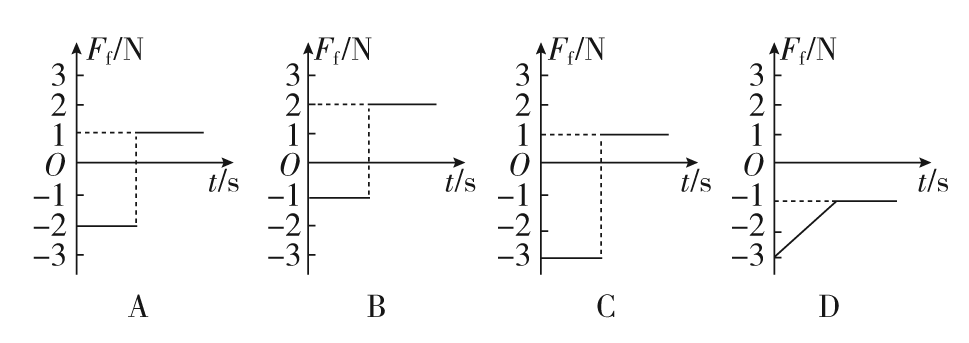
\includegraphics[scale=1]{./第1.2节匀变速直线运动的规律.pic/1} 所示木杆长5m,上端固定在某一点,由静止放开后让它自由落下(不计空气阻力),木杆通过悬点正下方20m处圆筒AB,圆筒AB长为5m,求:
\qitem 木杆经过圆筒的上端A所用的时间t1是多少?
\qitem 木杆通过圆筒AB所用的时间t2是多少?(取g=10\si{m/s^2})

6.在离地高h处,
沿竖直方向同时向上和向下抛出两个小球,它们的初速度大小均为v,
不计空气阻力,两球落地的时间差为
\choice[A]  $\frac{2v}{g}$ 
\choice[B]  $\frac{v}{g}$ 
\choice[C]  $\frac{2h}{v}$ 
\choice[D]  $\frac{h}{v}$ 

7.(可以略过)在以速度v匀速上升的电梯内竖直向上抛出一个小球,电梯内观察者看见
小球经时间t达到最高点,不计空气阻力,则有
\choice[A] 地面上的人所见小球抛出时的速度为v0=gt
\choice[B] 电梯中的人看见小球抛出时的速度为v0=gt
\choice[C] 地面上的人看见小球上升的最大高度为h= $\frac{1}{2}$ 
gt2
\choice[D] 地面上的人看见小球上升的时间也为t

\subsection{利用思维转换法巧解匀变速直线运动问题}


8.一物块(可看成质点)以一定的初速度从一光滑斜面底端A点上滑,最高可滑到C点,
已知AB是BC的3倍,如 \includegraphics[scale=1]{./第1.2节匀变速直线运动的规律.pic/3} 所示,已知物块从A至B所需时间为t0,则它从B经C再回到B,需要的时间是
\choice[A] t0
\choice[B]  $\frac{t0}{4}$ 
\choice[C] 2t0
\choice[D]  $\frac{t0}{2}$ 

9.如 \includegraphics[scale=1]{./第1.2节匀变速直线运动的规律.pic/5} 所示,一杂技演员用一只手抛球、接球,他每隔0.4s抛出一球,接到球便立即把球抛出。已知除抛、接球的时刻外,空中总有4个球,将球的运动近似看做是竖直方向的运动,球到达的最大高度是(高度从抛球点算起,取g=10\si{m/s^2})
\choice[A] 1.6m
\choice[B] 2.4m
\choice[C] 3.2m
\choice[D] 4.0m

10.如 \includegraphics[scale=1]{./第1.2节匀变速直线运动的规律.pic/7} 所示,在水平面上固定着三个完全相同的木块,一子弹以水平速度射入木块,若子弹在木块中做匀减速直线运动,当穿透第三个木块时速度恰好为零,则子弹依次射入每个木块时的速度比和穿过每个木块所用时间比分别为
\choice[A] v1:v2:v3=3:2:1
\choice[B] v1:v2:v3= $\sqrt{5}$ 
: $\sqrt{3}$ 
:1
\choice[C] Δt1:Δt2:Δt3=1: $\sqrt{2}$ 
: $\sqrt{3}$ 
\choice[D] Δt1:Δt2:Δt3=( $\sqrt{3}$ 
- $\sqrt{2}$ 
):
( $\sqrt{2}$ 
-1):1

11.从斜面上某一位置每隔0.1s释放一颗小球,在连续释放几颗后,对斜面上正在运
动着的小球拍下部分照片,如 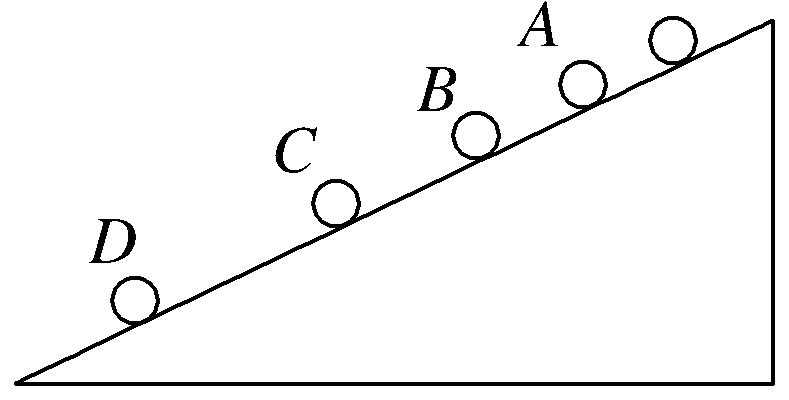
\includegraphics[scale=1]{./第1.2节匀变速直线运动的规律.pic/9} 所示。现测得xAB=15cm,xBC=20cm,已知小球在斜面上做匀加速直线运动,且加速度大小相同。
\qitem 求小球的加速度。
\qitem 求拍摄时B球的速度。
\qitem D、C两球相距多远?
\qitem A球上面正在运动着的小球共有几颗?
 
\end{document}
